\documentclass{article}

\input{include/libs.tex}
% pictures for states where players open offices modeled after the cards

\pgfmathsetmacro{\statewidth}{10}
\pgfmathsetmacro{\stateheight}{7.5}

\def\shapeState{(0,0) rectangle (\statewidth,\stateheight)}

\newcommand{\stateborder}{
    \draw \shapeState;
}

\newcommand{\statelabel}[1]{
    \node at (5,3.75) {\Huge #1};
}

\newcommand{\stateinstruction}[1]{
    \node at (5,1) {\large #1};
}

\newcommand{\statedebug}{
    \draw [step=1,help lines] (0,0) grid (\statewidth,\stateheight);
}


\begin{document}
\begin{center}
  \pagestyle{empty}
  \begin{tikzpicture}
    \stateborder
    \statelabel{Iowa}
    %\statedebug
  \end{tikzpicture}

  \vspace{2mm}
  \pagestyle{empty}
  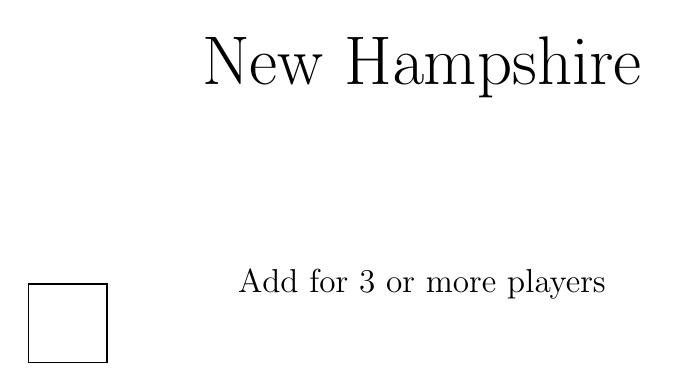
\begin{tikzpicture}
    \stateborder
    \statelabel{New Hampshire}
    \stateinstruction{Add for 3 or more players}
    %\statedebug
  \end{tikzpicture}

  \vspace{2mm}
  \pagestyle{empty}
  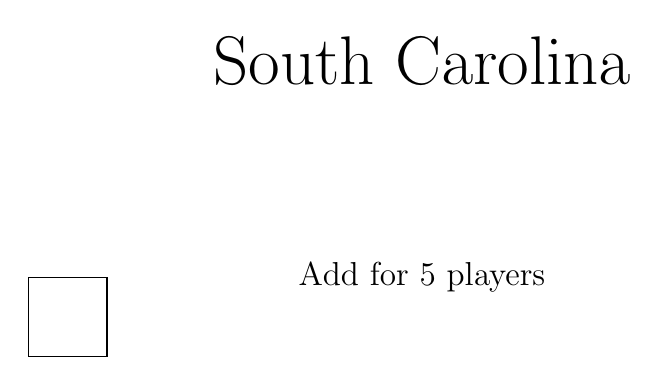
\begin{tikzpicture}
    \stateborder
    \statelabel{South Carolina}
    \stateinstruction{Add for 5 players}
    %\statedebug
  \end{tikzpicture}

\end{center}
\end{document}
